\documentclass{article}
\usepackage[utf8]{inputenc}
\usepackage[]{hyperref}
\usepackage[justification=justified]{caption}
\usepackage{tabulary}
\usepackage{color}
\usepackage{enumitem}
\newcolumntype{K}[1]{>{\centering\arraybackslash}p{#1}}

\author{
  Raatikka, Marko\\
  \texttt{marko.raatikka@aalto.fi}
  \and
  Lucas, Triefenbach\\
  \texttt{lucas.triefenbach@aalto.fi}
}
\title{Energy efficiency of HTTP2 over HTTP1.1 on the mobile web
\\
\vspace{5mm}
\large{CSE-E5440: Energy-efficient Mobile Computing\\Group C}
}
\date{\today}

\usepackage{natbib}
\usepackage{graphicx}

\begin{document}

\maketitle
\clearpage

\section{Part I}

\subsection{Introduction}
With the increasing computation power and connection speed of mobile phones in recent years, the amount of data flowing through the Internet to mobile end devices continues to grow. While web applications have become ever more complex and the amount of HTML, JavaScript and CSS required to render a web page increases, HTTP1.1 -- the prevailing transfer protocol of today's web -- has failed to keep up with the pace. One of the culprits of HTTP1.1 is that it can only handle one request per a TCP connection and that it can only have a certain maximum number of connections per host (5-8 connections depending on the browser). To work around these shortcomings developers have used techniques such as domain sharding (hosting assets across multiple domains), image spriting and inlining CSS \& JavaScript in the HTML. However, a transport layer problem can not be efficiently solved at the application level.

The work for a new version of HTTP protocol was set forth by Google in 2012 in the form an open networking protocol called SPDY. Later, in 2015, building on the work done for SPDY, HTTP2 was proposed as the future standard protocol. The biggest improvements HTTP2 introduces over HTTP1.1 are request/response multiplexing (to avoid a so called \emph{head-of-line blocking} inherent in HTTP1), header compression, prioritization of requests and server push mechanism. Web services are slowly migrating into adopting HTTP2, but as of today, only about 7\% of the websites have fully migrated to the new protocol. \citep{google-spdy}\citep{http2_stats}\citep{http2}

This work sets to study the impact of HTTP2 on mobile power consumption. Previous work on the topic has been done by \citep{previous_work}. However, this study focuses more on generating high traffic and mimicking common, real-life navigation patterns. Due to time constraints testing is limited to a single browser as opposed to testing across various versions. The content is organized as follows: Chapter \ref{chapter:design-implementation} describes the method used, the testbed environment and the test suite. Chapter \ref{chapter:results} continues by presenting the experiment results, which are later reviewed in Chapter \ref{chapter:discussion}. Last, an outline for the part II of the study is given.


\subsection{Design and Implementation}
\label{chapter:design-implementation}

The energy efficiency of the HTTP1.1 and HTTP2 protocols were measured by generating large amounts of network traffic. Three different web services were chosen as the target websites: \url{flickr.com}, \url{instagram.com} and \url{yahoo.com}. These web services were selected based on their popularity and support for HTTP2 clients (browsers). The original corpus included Facebook, Twitter and Weather.com as well. They were  however omitted from the corpus due to various reasons: the network traffic generated by Facebook was highly optimized, and therefore, it was assumed that it would not introduce any interesting statistical differences between HTTP1 and HTTP2. Twitter on the other hand was deemed too lightweight (consisting of mostly text-based content), while Weather.com suffered from peculiar latency issues when transmitting images over HTTP2 as shown by Figure \ref{fig:weather.com}.

\begin{figure}[h!]
\centering
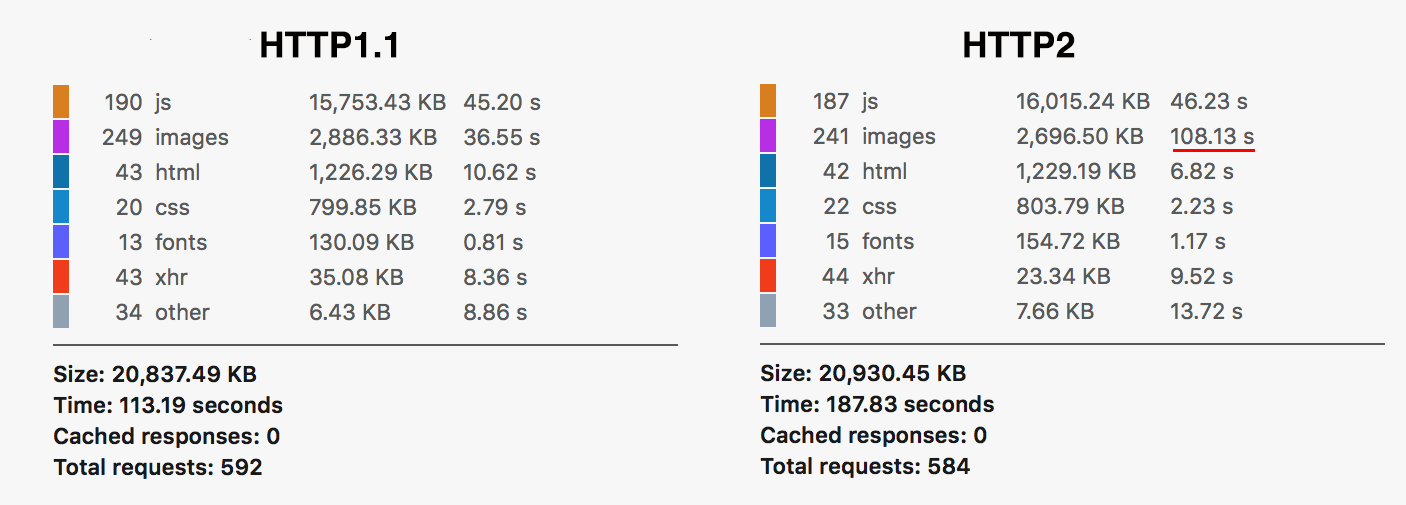
\includegraphics[width=\linewidth]{images/weathercom.png}
\caption{Weather.com was excluded from the final experiment corpus because it exhibited abnormally long response times when image assets were fetched over HTTP2. This was done the prevent introducing bias to the energy consumption measurements.}
\label{fig:weather.com}
\end{figure}

The experiment was conducted using Firefox (version 46.0) running on Samsung S4 (with Android 5.1.1). At the time of this writing, no other publicly available browser supports manually disabling HTTP2. The implementation of a robust and reproducible experiment environment required automation of the navigation logic. Browser automation frameworks Appium\footnote{Appium - \url{appium.io}} and Mozilla’s Robocop\footnote{Robocop - \url{https://wiki.mozilla.org/Auto-tools/Projects/Robocop}} were originally considered for this task. However, Appium lacked support for the Firefox browser, and Robocop -- Mozilla’s internal tool for testing Firefox on mobile -- missed up-to-date documentation. Thus, an alternative approach -- including the use of Android’s low level input API -- was taken. The utilization of the input API was inspired by an open-source energy consumption measurement framework called GreenMiner \citep{greenminer}, which uses this technique extensively.

The Android input API allows for the emulation of device gestures, and consequently, automation of browser navigation. The trade-off of this approach is that in some cases it requires root privilegs. Therefore the Samsung S4 used for the experiment was rooted using ClockworkMod recovery (version 6.0.4.7) and CyanogenMod (version 12). The upside of installing a custom ROM -- a customized OS image installed on the device's ROM memory -- like CyanogenMod is that any pre-installed Google services or bundled Samsung software are not included. This helped in minimizing any unwanted power consumption generated by these type of services running in the background unknowingly.

Monsoon Solutions' Power Monitor\footnote{\url{https://www.msoon.com/LabEquipment/PowerMonitor/}} was used for collecting the energy consumption data. The negative and positive terminals of the smartphone battery were connected to the power monitor using copper wire. The two reading terminals of the Samsung S4 battery were isolated with tape to allow the smartphone to be started using external power (the Power Monitor). The experiment scripts used for navigating to the different websites were implemented as Bash shell scripts. The scripts were transferred onto the device via USB using ADB (Android Debug Bridge). ADB also allowed orchestrating the execution of the test scripts from the laptop, so no human interaction was required while running the tests.

Prior to running the test suite different smartphone features that might have introduced noise (e.g. the energy consumption of background processes) were disabled. This included disabling automatic brightness, notifications, sounds, vibrations, widgets, lights and the phone's power saving features. Features enabled for experiment purposes were WiFi, Airplane mode and Developer options. The measurements were conducted in the Aalto open WiFi network during the late evening (22:00) to ensure low latency and minimal network congestion. All caching functionality of the Firefox browser was disabled to maximize network traffic (assets would always be fetched over the network). Crash reporting and monitoring capabilities of the browser were also disabled. The browser HTTP2 support was toggled on and off via the Firefox configuration interface (\url{about:config}). The cache and HTTP configuration flags used are listed in Table \ref{table:firefox_flags}. For further information the interested reader is referred to the MozillaZine Knowledge Base\footnote{MozillaZine Knowledge Base - \url{http://kb.mozillazine.org/}}.

\begin{table}[h!]
    \centering
    \caption{The Firefox configuration flags set in the experiment to disable caching and toggle HTTP2 support.}
    \label{table:firefox_flags}
    \begin{tabular}{l|c}
        \textbf{Flag} & \textbf{Value} \\
        browser.cache.check\_doc\_frequency & 1 \\
        browser.cache.disk.enable           & FALSE \\
        browser.cache.memory.enable         & FALSE \\
        network.http.spdy.enabled.http2     & TRUE/FALSE
    \end{tabular}
\end{table}

After connecting the smartphone and the laptop to the Power Monitor and opening the power measurement UI (Power Tool UI) the experiment was conducted as follows:

\begin{enumerate}
    \item Start the Power Monitor setting an output voltage of 3.7V and sampling rate of 5000Hz
    \item Boot the phone and ensure it has been configured as described above
    \item Connect the smartphone to the laptop via USB (for ADB communication)
    \item Install Firefox 46.0 via ADB and configure its settings as described above (partially automated)
    \item Execute the test suite \emph{n} number of times for either HTTP2 or HTTP1.1 (fully automated).
\end{enumerate}

Upon executing the test suite power monitoring is manually triggered via the Power Tool UI to record the energy consumption of the test runs. The rundown of the \emph{test suite} is as follows:

\begin{enumerate}
    \item Close stale instances of Firefox (if any)
    \item Ensure brightness is set to maximum and no screen dim is enabled
    \item Upload experiment scripts to the phone via ADB
    \item Wait $t_{bwt}$ seconds and start Firefox (opens at \emph{about:blank})
    \item Wait $t_{nwt}$ seconds and navigate to a target website
    \item Swipe down the page 5-6 times to force dynamic/lazily loaded content to be loaded waiting $t_{swt}$ seconds after each swipe
    \item Navigate to a subpage and wait $t_{nswt}$ seconds
    \item Repeat steps \textbf{6-7} for 4-6 different subpages
    \item Navigate to \emph{about:blank} and repeat steps \textbf{1-8} for each target website
    \item Wait $t_{nwt}$ seconds, close Firefox and wait another $t_{bwt}$ seconds before concluding the experiment.
\end{enumerate}

The wait times referred to above are given in Table \ref{table:wait_times}. The tap wait time $t_{twt}$ was used when tapping was required for loading more page content (e.g. tapping on a \emph{Load more} button). In addition to running the test suite to gather energy consumption metrics, the test suite was also run separately to capture network traffic (payload sizes, latency, number of requests) via the Firefox WebIDE\footnote{Firefox WebIDE - \url{https://developer.mozilla.org/en-US/docs/Tools/WebIDE}}.

\begin{table}[h!]
    \centering
    \caption{Wait time variables used in the experiment.}
    \label{table:wait_times}
    \begin{tabular}{l|c|l}
        \textbf{Variable} & \textbf{Duration (s)} & \textbf{Description} \\
        $t_{nwt}$   & 15    & Navigation wait time \\
        $t_{nswt}$  & 10    & Subpage navigation wait time \\
        $t_{bwt}$   & 5     & Base wait time \\
        $t_{swt}$   & 3     & Swipe wait time \\
        $t_{twt}$   & 2     & Tap wait time
    \end{tabular}
\end{table}

\subsection{Results}
\label{chapter:results}

The average network latency -- or Round Trip Time (RTT) -- and packet loss measured when connecting to the three target web services (Yahoo, Instagram, Flickr) via the Aalto open WiFi is presented in Table \ref{table:latency}. For both of the protocols (HTTP1.1 and HTTP2) the test suite was run three times. Figure \ref{fig:smoothed_power} visualizes the average power level for each of the (six) test runs. The results are plotted as a moving average using R\footnote{R: statistical computing framework - \url{https://www.r-project.org/}} and a generalized additive model (GAM) provided by the \emph{geom\_smooth()} function of the \emph{ggplot2}\footnote{ggplot2 - \url{http://docs.ggplot2.org/}} plotting library (version 2.1.0). As seen in the figure, it took a total of 400 seconds to complete a single run of the test suite.

Figure \ref{fig:average_power} presents the power levels of a test run done over HTTP1.1. The samples (x-axis) have been averaged over each 5000Hz interval (the sampling rate set for the Power Monitor). That is, each data point represents the average of a segment of 5000 data points (power levels). The moving (smoothed) average is included in the plot for comparison. Observations made based on the graph are labeled with letters \emph{A-E}, and discussed later in Chapter \ref{chapter:discussion}.

A summary of the mean power and total energy consumption of the three experiment runs for both HTTP2 and HTTP1.1 are given in Table \ref{table:energy_consumption}. The metrics are calculated for samples within the time frame of 24-395 seconds, which corresponds to the time when the first navigation is executed up until the time when navigating off to \emph{about:blank} after the last target website.

For more accurate analysis of the effect of the respective network traffic statistics, Figure \ref{fig:http2_network_traffic} provides a visualization of the payload sizes, latency and number of requests for both HTTP2 and HTTP1.1. This data is based on two individual runs done over both HTTP1.1 and HTTP2.

\begin{table}[h!]
    \centering
    \caption{RTT and packet loss experienced when being connected to the target websites via the Aalto open WiFi during the experiment.}
    \label{table:latency}
    \begin{tabular}{c|c|c|c}
         \textbf{Web service} & \textbf{RTT (ms)} & \textbf{RTT std. dev (ms)} & \textbf{Packet loss} \\
        Yahoo   & 158 & 32 & 4.7\% \\
        Instagram  & 116 & 10 & 0.3\% \\
        Flickr & 132 & 12 & 0.3\% \\
    \end{tabular}
\end{table}

\begin{figure}[h!]
\centering
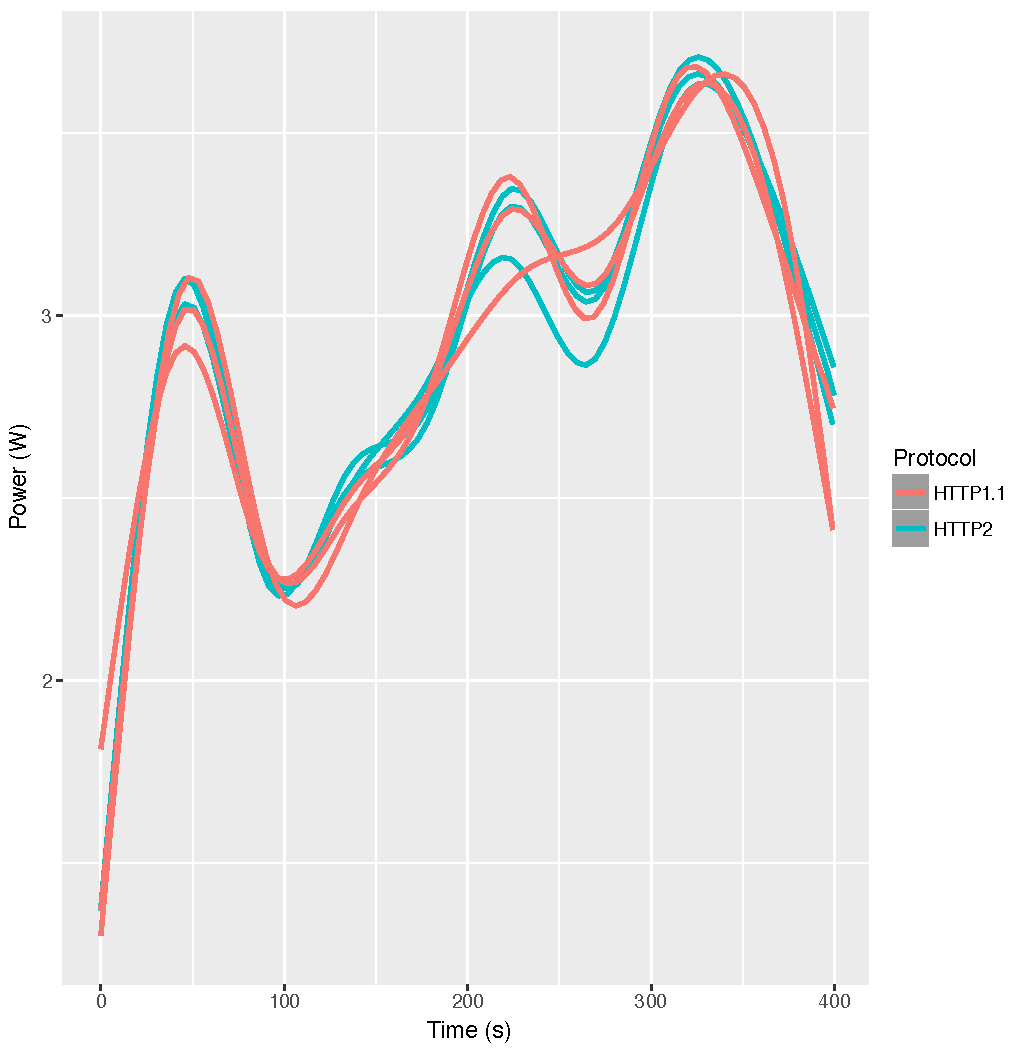
\includegraphics[width=\linewidth]{images/smoothed_power}
\caption{Smoothed average power draw of each six test runs over HTTP1.1 and HTTP2.}
\label{fig:smoothed_power}
\end{figure}

\begin{figure}[t]
\centering
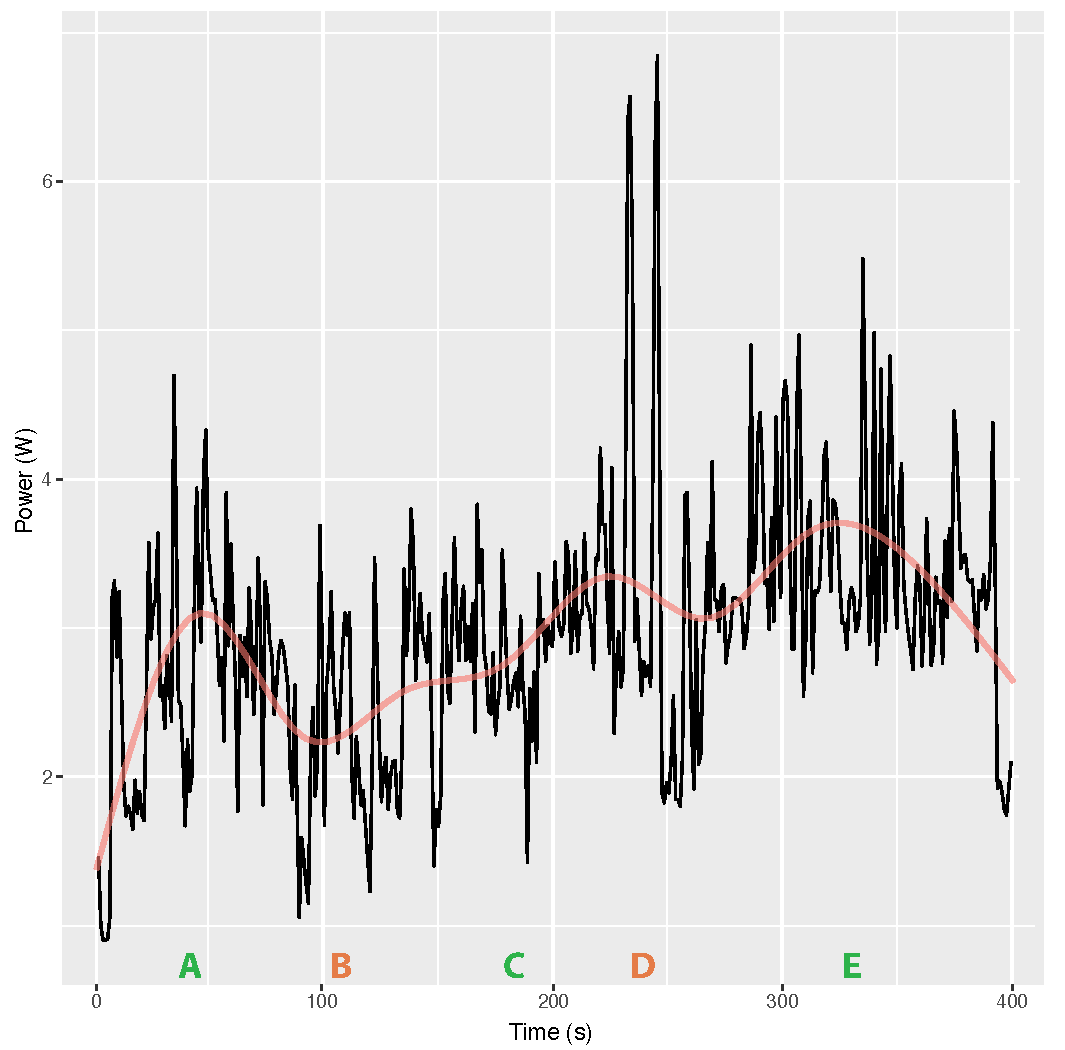
\includegraphics[width=\linewidth]{images/average_power}
\caption{Average power draw and smoothed average of a test run done over HTTP1.1.}
\label{fig:average_power}
\end{figure}

\begin{table}[h!]
    \centering
    \caption{Energy consumption of HTTP1.1 and HTTP2 over the time frame of 24-395 seconds (from the first navigation up until the exit navigation).}
    \label{table:energy_consumption}
    \begin{tabular}{c|c|c}
        & \textbf{HTTP1.1} & \textbf{HTTP2}  \\
        Mean (W)   & 2.987 & 2.995 \\
        Std.dev (W) & 0.984 & 1.007 \\
        Total (J)  & 1114.2 & 1117.2 \\
    \end{tabular}
\end{table}

\begin{figure}[h!]
\centering
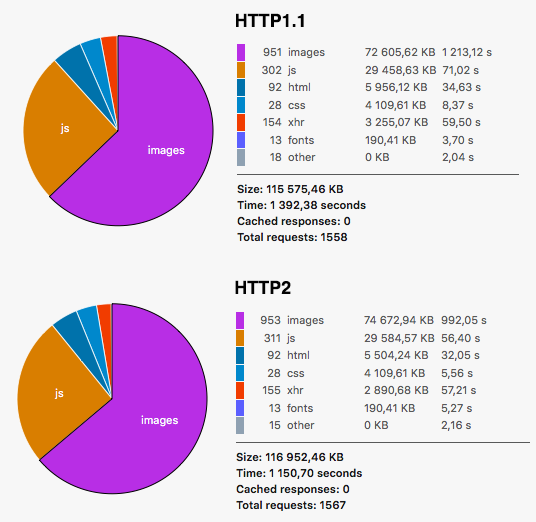
\includegraphics[width=\linewidth]{images/http2_consumes.png}
\caption{The network traffic statistics for single test suite runs over HTTP1.1 and HTTP2.}
\label{fig:http2_network_traffic}
\end{figure}

\clearpage

\subsection{Discussion}
\label{chapter:discussion}

One of the early goals was to compare the energy consumption of the HTTP protocols in different network (latency) conditions as in \cite{previous_work} it was found that significant difference in the energy consumption was observed in the vincinity of 250ms, but not on lower or higher latencies. The objective was to test if this indeed was the case. Unfortunately however, implementing a setup for reliable latency adjustment (e.g proxying the traffic via VPN) was not done due to time constraints. Therefore, experiments were only performed under the Aalto open WiFi in part I of this study. An alternative approach would have been to force the phone to use a 2G or 3G network. However, 2G proved too unreliable (high packet loss), while 3G actually provided relatively low latency (150ms) similar to that of the Aalto open WiFi connection -- most likely due to the nearby location of the network antenna.

As seen in Table \ref{table:latency} \url{yahoo.com} exhibited higher latency and packet loss. This was believed to be due to the fact that the pages include a relatively high number of ads from various mobile advertisement providers. Furthermore, it can be argued that the CDNs (Content Delivery Network) for Yahoo are less ideally positioned then that of Instagram and Flickr. However, the average latencies are still within a reasonable range (116-158ms) to assume a low latency test conditions.

Figure \ref{fig:smoothed_power} shows that the energy consumption difference between the two protocols is minimal. Three runs for both of the protocol is not however enough to draw conclusions. The bump in the average power level for \url{yahoo.com} (also seen in the two power spikes in Figure \ref{fig:average_power}) can be attributed to \emph{layout trashing} (by the GPU) observed when swiping down \url{https://yahoo.com/style} on mobile. Thus, it was decided that \emph{/style} be omitted from the corpus for part II experiments. One of the HTTP1.1 runs did not seem to exhibit this ``spiky'' behaviour, though. This only goes to show how important it would have been to perform more test runs to minimize the effects of anomalies.

Some interesting observations can be made from the graph in Figure \ref{fig:average_power}. First, it can be seen (from the raw data) that the base power of the phone is around 1.2W. Launching and running Firefox increases the base power draw to the vincinity of 1.65W (12-24 seconds). Labels \emph{A}  and \emph{B} represent the power draw when browsing \url{instagram.com} (24-120 seconds). The reason why the power level suddenly drops well below 2W twice (\emph{B}) was due to the fact that the page visited (\url{https://flickr.com/photos/tags}) was light on content, and was actually navigated to \emph{twice}, consecutively. As the URL would not change when navigated to the second time, Firefox was smart enough to not load the page preserving energy in the process. The fact that this subpage was visited twice in a row was an implementation bug missed by the authors when conducting the tests (fixed in part II).

Label \emph{C} and \emph{D} represent the power draw when browsing \url{flickr.com} (at 135-250 seconds). The spikes (\emph{D}) were due to layout trashing as referred to earlier. Last, label \emph{E} represents the browsing of \url{instagram.com} (at 260-395 seconds). Judging by the graph, it seems as if Instagram would be the most energy inefficient. However, as the order of target websites in the corpus was not randomized, such conclusions can not be drawn. It might very well be that the progressive increase in the power draw is due to increasing device temperature, or Firefox's excess allocation of memory and/or processes over time.

The energy consumption results summarized in Table \ref{table:energy_consumption} show that the consumption was virtually identical between HTTP1.1 and HTTP2 across the test runs. However, Figure \ref{fig:http2_network_traffic} suggests that HTTP2 had better network performance. For example, HTTP2 spent 20\% less time on average for fetching assets. Thus, it could be argued that HTTP2 had higher energy utility -- 22\% higher kB/s/J based on Table \ref{table:energy_consumption} and Figure \ref{fig:http2_network_traffic}.

An effort was given to follow the best practices of software energy experimentation as per \textbf{ENERGISE}\footnote{Software energy experimentation best practices: \url{https://github.com/ds4se/chapters/blob/c6f960b5955ef835752f265eed7337ff51cf35e0/abramhindle/energymining.md\#lets-energise-your-software-energy-experiments}} -- a mnemonic coined by the authors of \cite{greenminer}. Due to time constraints the tests were run only on one Firefox version (46.0). Moreover, only three test runs were done for both protocols, which clearly is not enough to draw any statistically significant conclusions. However, in other aspects of the ENERGISE practices the experiment was conducted to the authors' best ability. Especially, the automation of the test suite was a significant achievement, which helped in improving and adjusting the testbed for part II of this study.

\section{Part II}

Based on part I observations and feedback the following improvements/adjustments were made to the testbed:

\begin{itemize}
    \item increase of test run count to 10 for better confidence
    \item traffic throttling via a VPN for simulating high latency conditions
    \item URL manifest generation and more in-depth network traffic metrics
    \item test suite adjustments:
        \begin{itemize}
        \item changed test suite to be run separately for each target website instead of profiling them all in one go
        \item omitted \url{yahoo.com/style} from the corpus
        \item removed duplicate navigation to \url{flickr.com/photos/tags}
        \end{itemize}
\end{itemize}

High latency conditions were simulated by tunneling the smartphone network traffic via a VPN located in US west coast. The average ping measured varied around $300\pm60$ms. Accurate high latency RTTs are provided in Table \ref{table:network-stats}.

The goal of part II of the assignment was to propose solutions for improving the energy-efficiency of the mobile application/service studied in part I. Since this study investigated the performance HTTP protocols rather than an individual application/service, the solution is proposed in form of HTTP2 best practices for application developers. The rest of this paper is organized as follows: Chapter \ref{chapter:results-part2} presents the results of part II after applying the aforementioned testbed improvements. Chapter \ref{chapter:discussion-part2} continues with a dicussion of the results and presents an outline for HTTP2 best practices. Last, Chapter \ref{chapter:conclusions} concludes with a summary of the study and suggestions for future work.

\subsection{Results}
\label{chapter:results-part2}

In part II energy consumption and traffic metrcis were captured separately for each target website so that any increase in device temperature or tail energy from previous activity would not be reflected on the power draw of the consecutive run. The \emph{Visit Duration} given in Table \ref{table:url_manifest} denotes the time between the initial navigation to and the exit navigation from a target website. All results have been computed based on this time frame.

\begin{table}[h!]
    \caption{URL manifest; the target websites and subpages visited. The payload and RTT values are the average of all the runs (HTTP1.1 and HTTP2) executed in low latency conditions.}
    \label{table:url_manifest}
    \begin{tabular}{lK{2.6cm}K{2.5cm}K{2.25cm}}
        \textbf{Site} & \textbf{Visit Duration} (s) & \textbf{Avg. Payload} (kB) & \textbf{Avg. RTT} (ms) \\
        \hline \vspace{-3mm}\\
        \textbf{https://flickr.com} & 170 & 64 261 & $131.6\pm6.6$ \\
        \hspace{1em} /explore \\
        \hspace{1em} /photos/tags/primavera \\
        \hspace{1em} /photos/tags/amazing \\
        \hspace{1em} /photos/tags/rural \\
        \hspace{1em} /photos/tags/brazil \vspace{1mm}\\
        \textbf{https://instagram.com} & 200 & 32 937 & $112.7\pm4.7$ \\
        \hspace{1em} /nhl \\
        \hspace{1em} /binghuiliu \\
        \hspace{1em} /jordanspieth \\
        \hspace{1em} /warriors \\
        \hspace{1em} /nba \\
        \hspace{1em} /ufc \vspace{1mm}\\
        \textbf{https://yahoo.com} & 150 & 20 162 & $133.3\pm8$ \\
        \hspace{1em} /tech \\
        \hspace{1em} /news \\
        \hspace{1em} /business \\
        \hspace{1em} /tv \vspace{1mm}\\
    \end{tabular}
\end{table}

\begin{figure}[h!]
    \centering
    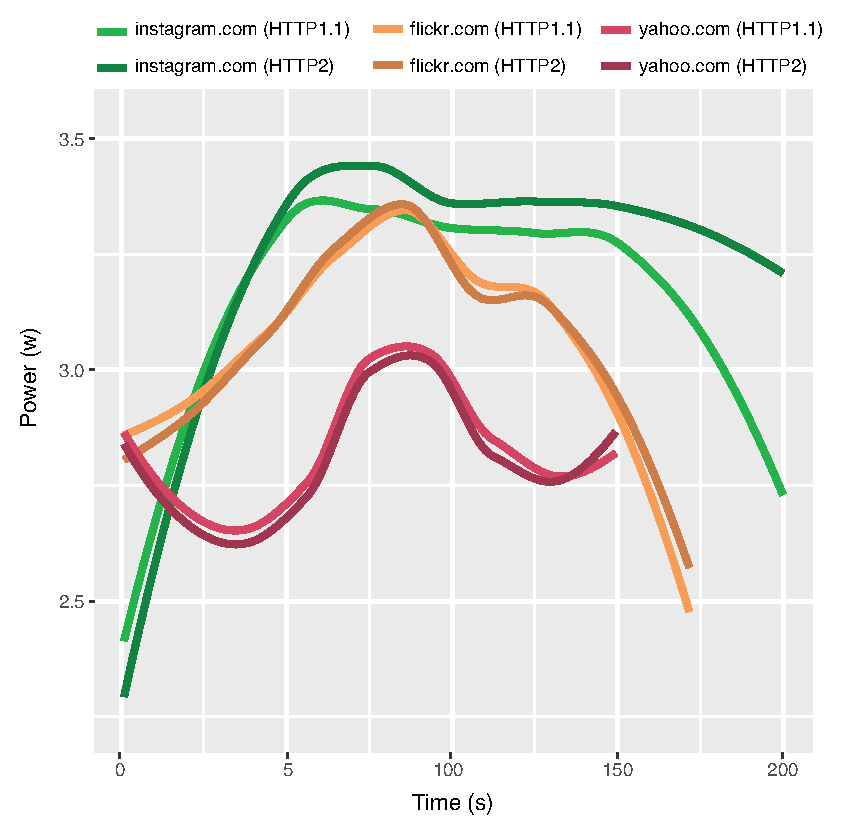
\includegraphics[width=\linewidth]{images/average}
    \caption{Average power draw of HTTP1.1 and HTTP2 per target website (low latency, 100-130ms).}
    \label{fig:average}
\end{figure}

\begin{figure}[h!]
    \centering
    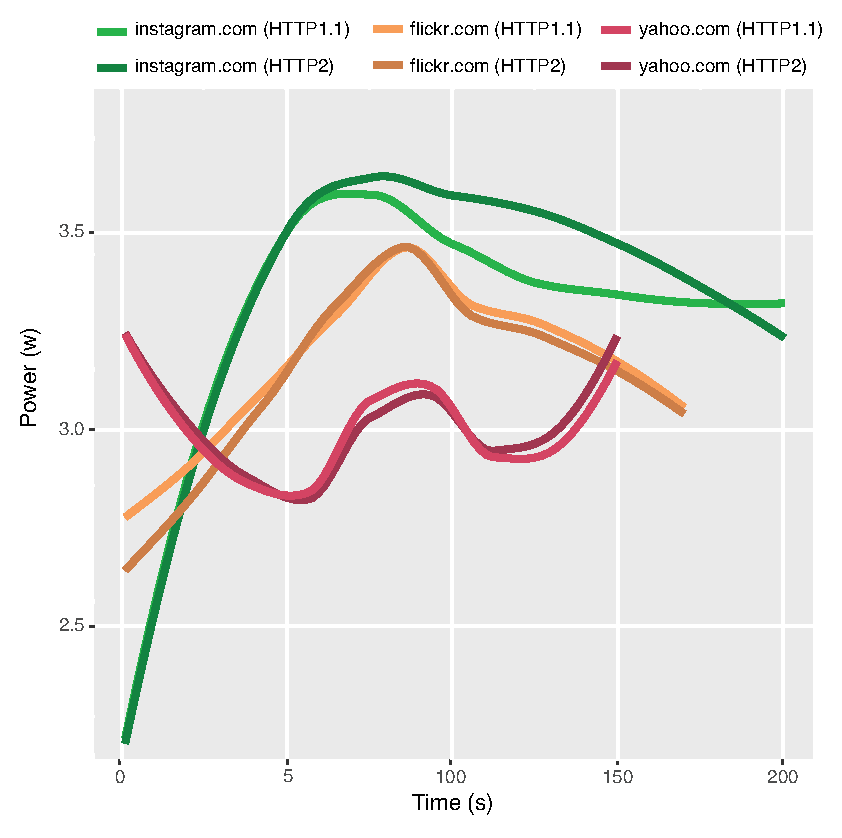
\includegraphics[width=0.98\linewidth]{images/average-vpn}
    \vspace{-3mm}
    \caption{Average power draw of HTTP1.1 and HTTP2 per target website (high latency, 300ms).}
    \label{fig:average-vpn}
\end{figure}

\begin{table}[h!]
    \caption{Energy consumption of the target websites over HTTP1.1 \& HTTP2. HL denotes high latency conditions of 300ms RTT (110-130ms otherwise).}
    \label{table:energy_consumption_part2}
    \vspace{-3mm}
    \begin{tabular}{|l|K{2.25cm}|K{2.75cm}|K{2.75cm}|}
        \hline
        \textcolor{blue}{HTTP1.1} / \textcolor{red}{HTTP2} & \textbf{Total energy} (J) & \textbf{Power average} (W) & \textbf{Power std.dev} (W) \\ \hline
        Flickr & \textcolor{blue}{519.7} / \textcolor{red}{520.1}  &\textcolor{blue}{3.075} / \textcolor{red}{3.077}  &
        \textcolor{blue}{0.832} / \textcolor{red}{0.748}  \\ \hline
        Flickr (HL) & \textcolor{blue}{659.8} / \textcolor{red}{532.3}  &\textcolor{blue}{3.315} / \textcolor{red}{3.149}  &
        \textcolor{blue}{0.841} / \textcolor{red}{0.797}  \\ \hline

        Instagram & \textcolor{blue}{631.4} / \textcolor{red}{646.2} & \textcolor{blue}{3.172} / \textcolor{red}{3.247} & \textcolor{blue}{0.705} / \textcolor{red}{0.754} \\ \hline

        Instagram (HL) & \textcolor{blue}{659.8} / \textcolor{red}{670.0} & \textcolor{blue}{3.315} / \textcolor{red}{3.366} & \textcolor{blue}{0.841} / \textcolor{red}{0.857} \\ \hline

        Yahoo & \textcolor{blue}{417.4} / \textcolor{red}{413.9} &\textcolor{blue}{2.801} / \textcolor{red}{2.778}  & \textcolor{blue}{0.624} / \textcolor{red}{0.597}  \\ \hline
        Yahoo (HL) & \textcolor{blue}{447.6} / \textcolor{red}{446.6} &\textcolor{blue}{3.004} / \textcolor{red}{2.997}  & \textcolor{blue}{0.586} / \textcolor{red}{0.611}  \\ \hline
    \end{tabular}
\end{table}

\begin{table}[h!]
    \caption{Network traffic statistics and energy utility (kB/s/J) for each target website during the (low latency) test runs. The average latency and energy utility under high latency conditions are also included for comparison.}
    \label{table:network-stats}
    \begin{tabular}{|l|K{2.7cm}|K{2.8cm}|K{2.5cm}|}
        \hline
        \textcolor{blue}{HTTP1.1} / \textcolor{red}{HTTP2} & \textbf{Flickr} & \textbf{Instagram} & \textbf{Yahoo} \\ \hline
        Total Payload (kB) & \textcolor{blue}{63669} / \textcolor{red}{64853}  & \textcolor{blue}{33210} / \textcolor{red}{32664}  &
        \textcolor{blue}{19833} / \textcolor{red}{20491}  \\ \hline
        Total Response Time (s) & \textcolor{blue}{1135} / \textcolor{red}{936}  &\textcolor{blue}{117} / \textcolor{red}{170}  &
        \textcolor{blue}{127} / \textcolor{red}{119}  \\ \hline

        Number of Requests & \textcolor{blue}{587} / \textcolor{red}{606} & \textcolor{blue}{469} / \textcolor{red}{464} & \textcolor{blue}{511} / \textcolor{red}{509} \\ \hline

        Total Bit Rate (kB/s) & \textcolor{blue}{56.1} / \textcolor{red}{69.3} & \textcolor{blue}{283.8} / \textcolor{red}{192.1} & \textcolor{blue}{156.2} / \textcolor{red}{172.2} \\  \hline

        Image Bit Rate (kB/s) & \textcolor{blue}{8.1} / \textcolor{red}{10.2} &\textcolor{blue}{51.9} / \textcolor{red}{33.2}  & \textcolor{blue}{18.8} / \textcolor{red}{24.4}  \\ \hline

        JS Bit Rate (kB/s) & \textcolor{blue}{59.7} / \textcolor{red}{64.3} &\textcolor{blue}{354.5} / \textcolor{red}{301.8}  & \textcolor{blue}{87.2} / \textcolor{red}{87.8}  \\ \hline

        Energy Utility (kB/s/J) & \textcolor{blue}{0.108} / \textcolor{red}{0.133} & \textcolor{blue}{0.449} / \textcolor{red}{0.297} & \textcolor{blue}{0.374} / \textcolor{red}{0.416} \\ \hline

        Latency / RTT (ms) & $131.6\pm6.6$\newline(HL: $306\pm50.5$)    & $112.7\pm4.7$\newline(HL: $295.6\pm56.3$) & $133.3\pm8$\newline(HL: $304\pm77.8$) \\ \hline
    \end{tabular}
\end{table}

\begin{figure}[h!]
    \centering
    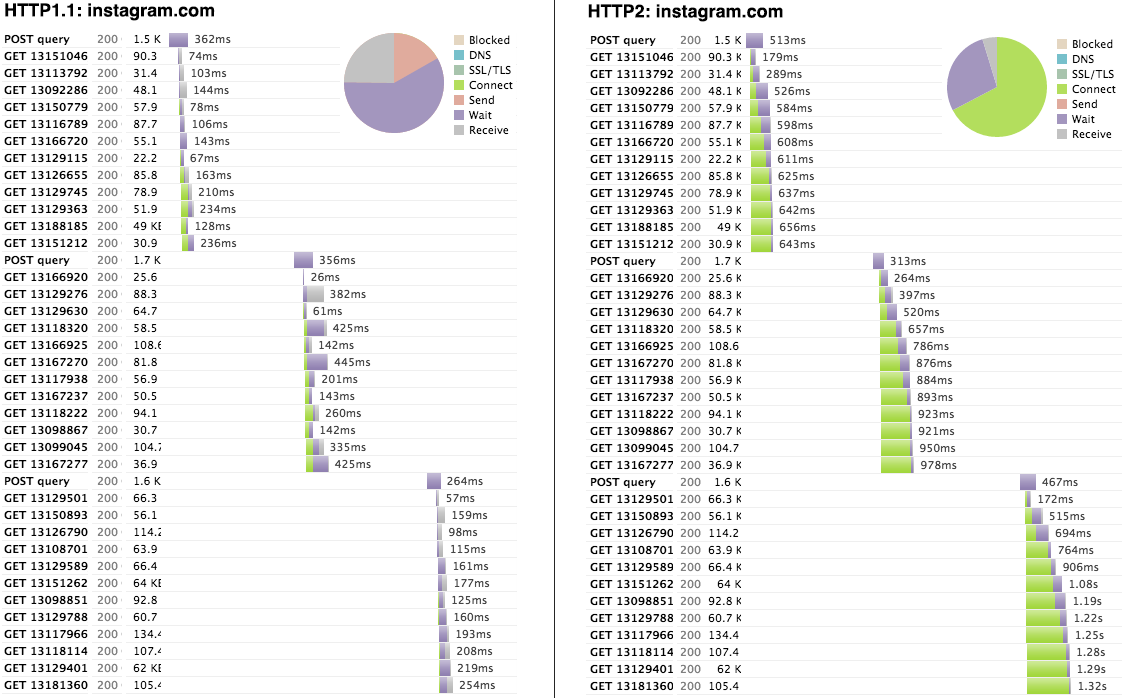
\includegraphics[width=1.1\linewidth]{images/waterfall_instagram}
    \caption{A snippet of the network waterfall for \url{instagram.com/warriors} when browsed over HTTP1.1 and HTTP2 with Firefox 46.0 and Google Chrome 50.0. Browsing \url{instagram.com} over HTTP2 on Firefox 46.0 seemed to suffer from long delays in establishing a TCP connection when fetching image assets.}
    \label{fig:instagram-waterfall}
\end{figure}

\clearpage

\subsection{Discussion}
\label{chapter:discussion-part2}

Initially for part II measurements an attempt was made to manually turn on Android's \emph{Performance Governor} during the experiments to ensure a more predictable, base CPU power draw. However, this did not turn out to be possible as is lead to instable, laggy behaviour.

The following question were laid out based on part I results:
\\
\begin{itemize}[label={}]
    \item \emph{Did you get exactly the same content every time?}\\\\
    Slight variance in the total payload size and number of requests for each of the test runs was observed. This was likely due to varying network conditions both in the client's and the server's end. However, based on the raw data and author's observations these variations were minimal enough to be cancelled out by having the test suite executed multiple times (10). No attempt was made for automatically detecting significant changes in the network conditions during the experiment. However, nothing in the final data pointed to any discrepancies. Only a couple of test runs were re-run as the power draw was noticeably different (contained anomalies).\\

    \item \emph{What are the potential causes of the difference in energy consumption? Do they transfer data in a different way?}\\\\
    HTTP2 is able to handle multiple request more efficiently by multiplexing them (using streams). Requests made on the same connection can be responded to out of order, which means the client can use a single TCP connection to make all their requests. When properly supported by both the client and the server, this results in reduced memory, network and CPU load for both parties as a new TCP connection need not be opened for each request. The respective payload size for HTTP2 is slightly bigger due to the higher number of required HTTP header fields.\\
\end{itemize}

Tables \ref{table:network-stats} and \ref{table:energy_consumption_part2} show that HTTP2 provides better energy utility, especially in the case of high latency conditions. This was not however the case with Instagram, which -- much like Weather.com in part I of the study -- exhibited longer response times when transferring image assets. This in turn lead to higher energy consumption in both low and high latency scenarios (even though in high latency conditions the difference narrowed down a bit) as the TCP connections were kept alive for a longer time. This discrepancy was believed to have been caused by an incompability between the client's (Firefox 46.0) and the server's HTTP2 implementation. The disabling of caching might also have affected the functionality of the server in unexpected ways. Analysing the network traffic waterfall of e.g. \url{instagram.com/warriors} as depicted in Figure \ref{fig:instagram-waterfall} shows that Firefox 46.0 seemed to suffer from long delays in establishing a TCP connection over HTTP2. Google Chrome (50.0) did not exhibit this behaviour, which further supports the aforementioned assumption.

% HTTP2 Best Practices (http://blog.scottlogic.com/2014/11/07/http-2-a-quick-look.html)

\subsection{Conclusions}
\label{chapter:conclusions}

Part II measurements alone took almost 7 hours to run (average test run duration of 200s $\times$ 120 test runs). It would have been impractical to do the measurements manually, so automation of the test suite was crucial for ensuring accurate and reproducable data capture.

Conclusion: in low latency conditions HTTP2 has little impact, whereas in high latency conditions it can be result in significant energy savings for high content websites. HTTP2 is still in its infancy and requires careful configuration. As such, it can even increase energy consumption if compability with existing systems/browsers is not tested for.

% An outline for future work/experiments

\bibliographystyle{plain}
\bibliography{references}
\end{document}
